\documentclass{article}

\usepackage{graphicx}
\usepackage{tikz}
\usepackage{tikzsymbols}
\usetikzlibrary{calc,patterns,shapes.geometric}
\pagestyle{empty}
\usepackage[margin=0pt]{geometry}
\geometry{papersize={14in,12in}}

\def\centerarc[#1](#2)(#3:#4:#5){\draw[#1] ($(#2)+({#5*cos(#3)},{#5*sin(#3)})$) arc (#3:#4:#5);}

\begin{document}
	\begin{figure}
		\centering
		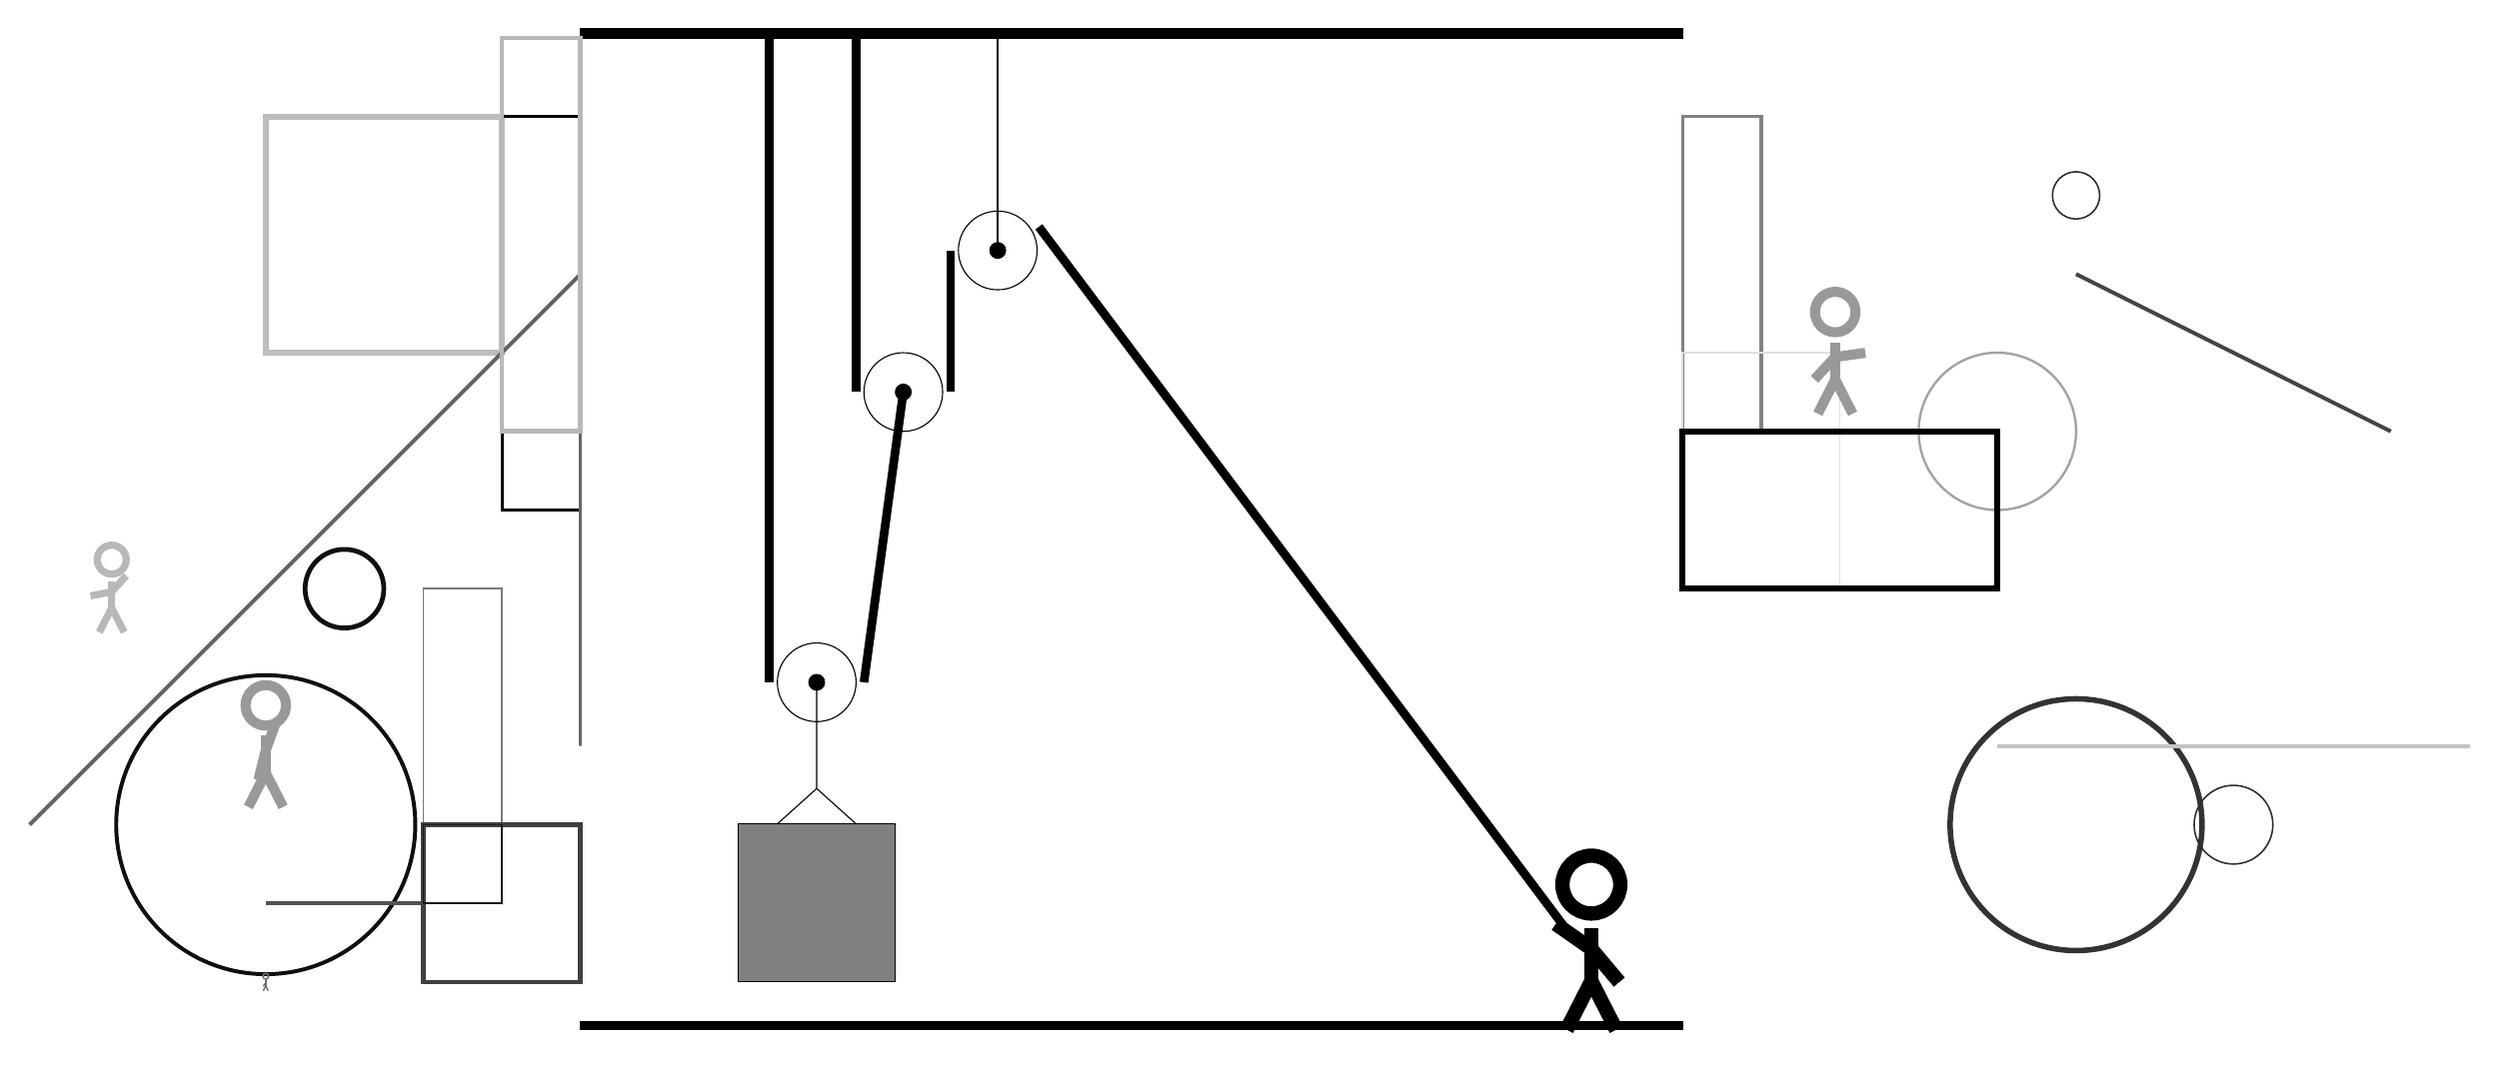
\begin{tikzpicture}
			%%%%% START %%%%%
			
			\draw[fill=black] (-2, 9) rectangle (12, 9.125);
			
			\draw (1, 0.81) circle (0.5);
			\draw[fill=black] (1, 0.81) circle (0.1);
			
			\draw[line width=0.7mm, color=black!26] (-3, 5) rectangle (-6, 8);
			
			\draw[line width=0.4mm, color=black!100] (-2, 8) rectangle (-3, 3);
			\draw [line width=0.5mm, color=black!94](-6, -1) circle (1.9);
			\draw[line width=0.4mm, color=black!49] (12, 8) rectangle (13, 4);
			\draw [line width=0.6mm, color=black!94](-5, 2) circle (0.5);
			\draw[line width=0.2mm, color=black!13] (12, 5) rectangle (14, 2);
			\draw [line width=0.7mm, color=black!80](17, -1) circle (1.6);
			\draw[line width=0.5mm, color=black!23](16, 0) -- (22, 0);
			\draw[line width=0.2mm, color=black!52] (-3, 2) rectangle (-4, -2);
			\draw[line width=0.5mm, color=black!68](-4, -2) -- (-6, -2);
			\node[line width=0.5mm, color=black!40] at (-6, 0) {\Strichmaxerl[7][76][70]};
			\draw[line width=0.6mm, color=black!75] (-2, -1) rectangle (-4, -3);
			\draw [line width=0.3mm, color=black!36](16, 4) circle (1.0);
			
			\draw[line width=0.5mm, color=black!61](-2, 6) -- (-9, -1);
			\draw[line width=0.7mm, color=black!28] (14, 2) rectangle (14, 2);
			\node[line width=0.4mm, color=black!40] at (14, 5) {\Strichmaxerl[7][47][8]};
			
			\draw[line width=0.4mm, color=black!60] (-2, 7) rectangle (-2, 0);
			\draw[line width=0.6mm, color=black!28] (-2, 4) rectangle (-3, 9);
			\draw [line width=0.2mm, color=black!82](19, -1) circle (0.5);
			\draw[line width=0.7mm, color=black!100] (12, 2) rectangle (16, 4);
			\node[line width=0.2mm, color=black!56] at (-6, -3) {\Strichmaxerl[1][55][82]};
			\draw[line width=0.5mm, color=black!73](17, 6) -- (21, 4);
			
			\draw [line width=0.2mm, color=black!82](17, 7) circle (0.3);
			\draw[line width=0.2mm, color=black!90] (-4, -1) rectangle (-3, -2);
			\node[line width=0.5mm, color=black!28] at (-8, 2) {\Strichmaxerl[5][11][48]};
			
			
			\draw (2.1, 4.5) circle (0.5);
			\draw[fill=black] (2.1, 4.5) circle (0.1);
			
			\draw (3.3, 6.3) circle (0.5);
			\draw[fill=black] (3.3, 6.3) circle (0.1);
			\draw[thick] (3.3, 6.3) -- (3.3, 9);
			
			\draw (1, 0.81) -- (1, -0.54) -- (0.5, -0.99) -- (1.5, -0.99) -- (1, -0.54);
			\draw[fill=black!50] (0, -0.99) rectangle (2, -2.99);
			
			\draw[line width=1.1mm] (0.4, 9) -- (0.4, 0.81);
			\centerarc[line width=1.1mm](1, 0.81)(180:360:0.6);
			\draw[line width=1.1mm](1.6, 0.81) -- (2.1, 4.5);
			\draw[line width=1.1mm] (1.5, 9) -- (1.5, 4.5);
			\centerarc[line width=1.1mm](2.1, 4.5)(180:360:0.6);
			\draw[line width=1.1mm](2.7, 4.5) -- (2.7, 6.3);
			\centerarc[line width=1.1mm](3.3, 6.3)(30:180:0.6);
			\draw[line width=1.1mm] (3.822, 6.6) -- (10.5, -2.3);
			
			\node at (10.8, -2.5) {\Strichmaxerl[10][-35][-50]};
			
			\draw[fill=black] (-2, -3.5) rectangle (12, -3.6);
			
			%%%%% END %%%%%
		\end{tikzpicture}
	\end{figure}	
\end{document}